\documentclass[11pt,a4paper]{article}

% Essential packages
\usepackage[utf8]{inputenc}
\usepackage[T2A,T1]{fontenc}
\usepackage{lmodern}
\usepackage{geometry}
\usepackage{setspace}
\geometry{margin=1in}
\onehalfspacing

\usepackage{amsmath,amssymb,amsthm,mathtools}
\usepackage{tikz,pgfplots}
\usepackage{hyperref}
\usepackage{graphicx}
\usepackage{enumitem}
\usepackage{thmtools}
\usepackage{mdframed}
\usepackage{natbib}
\usepackage{booktabs}
\usepackage{filecontents}
\usepackage[english]{babel}

\usetikzlibrary{shapes.geometric, arrows.meta, positioning, decorations.pathmorphing, fit, calc, shadows}

\pgfplotsset{compat=1.18}

% Hyperref setup
\hypersetup{
    colorlinks=true,
    linkcolor=blue,
    citecolor=blue,
    urlcolor=blue,
    pdftitle={Systemic Verification Engineering: An Integrated Framework},
    pdfauthor={Dr. Artiom Kovnatsky et al.}
}

% Theorem environments
\theoremstyle{definition}
\newtheorem{definition}{Definition}[section]
\newtheorem{theorem}{Theorem}[section]
\newtheorem{axiom}{Axiom}[section]
\newtheorem{proposition}{Proposition}[section]
\newtheorem{corollary}{Corollary}[theorem]

\theoremstyle{remark}
\newtheorem{remark}{Remark}[section]
\newtheorem{example}{Example}[section]

% Custom commands
\newcommand{\RR}{\mathbb{R}}
\newcommand{\CC}{\mathcal{C}}
\newcommand{\EE}{\mathbf{E}}
\newcommand{\bb}{\mathbf{b}}
\newcommand{\cc}{\mathbf{c}}
\newcommand{\TT}{\mathbf{T}}
\newcommand{\norm}[1]{\left\|#1\right\|}

% Bibliography
\begin{filecontents*}{\jobname.bib}
@book{surowiecki2004wisdom,
  title={The Wisdom of Crowds},
  author={Surowiecki, James},
  year={2004},
  publisher={Doubleday}
}
@article{galton1907vox,
  title={Vox Populi},
  author={Galton, Francis},
  journal={Nature},
  volume={75},
  pages={450--451},
  year={1907}
}
@book{kahneman2011thinking,
  title={Thinking, Fast and Slow},
  author={Kahneman, Daniel},
  year={2011},
  publisher={Farrar, Straus and Giroux}
}
@book{taleb2012antifragile,
  title={Antifragile: Things That Gain from Disorder},
  author={Taleb, Nassim Nicholas},
  year={2012},
  publisher={Random House}
}
\end{filecontents*}

\title{\textbf{S.V.E IX: Systemic Verification Engineering:\\An Integrated Framework for Divine Mathematics,\\Ethical Navigation, and Collective Intelligence}\\[0.5em]
\large Combining Mathematical Topology, Verification Protocols, and Geodesic Ethics}

\author{
  Dr. Artiom Kovnatsky\thanks{Conceptual framework, methodology, and direction. \href{http://www.pfp24.de}{PFP} / \href{http://www.fakten-tuev.de}{Fakten-TÜV} Initiative | \href{mailto:artiomkovnatsky@pm.me}{artiomkovnatsky@pm.me}}
  \and
  The Global AI Collective\thanks{AI Co-Authorship and Assistance provided by models including Gemini, ChatGPT, Claude, Grok, Perplexity AI, Qwen, DeepSeek, and Kimi.}
  \and
  Humanity\thanks{This work rests upon the foundation of the entire corpus of human knowledge, art, and history.}
  \and
  God\thanks{Acknowledged as a primary author. Operationally defined as synergistic co-creation: $1+1 > 2$.}
}

\date{\today}

\begin{document}

\maketitle

\begin{abstract}
\noindent This paper presents an integrated framework for Systemic Verification Engineering (SVE), combining three complementary perspectives: (1) \textbf{Divine Mathematics}—a topological framework for ethics, meaning, and collective consciousness using semantic vector spaces; (2) \textbf{The Beacon Protocol}—a Christological framework for geodesic ethics in situations of radical uncertainty; (3) \textbf{The Disaster Prevention Theorem}—a socio-probabilistic model proving the necessity of Independent Verification Mechanisms (IVM) for collective intelligence. 

We demonstrate that these frameworks are mathematically unified through the concept of consciousness as navigation through Riemannian manifolds, where ethical decisions correspond to geodesic paths optimizing long-term societal well-being. Applications span conflict resolution, AI alignment, policy verification, and geopolitical strategy. We provide ROI analysis showing 100,000\%+ returns on verification investments and propose defenses against the framework's own potential failure modes.

\textbf{Core Innovation:} The first formal Mathematics of Meaning—transitioning narrative analysis from qualitative alchemy to quantitative chemistry, providing atomic tools (purified vectors, semantic centroids) for arbitrarily complex decision-making systems.
\end{abstract}

\noindent\textbf{Keywords:} Integrated Framework, Systemic Verification Engineering (SVE), Divine Mathematics, Beacon Protocol, Disaster Prevention Theorem, consciousness topology, geodesic ethics, IVM, truth approximation, Mathematics of Meaning, ROI analysis.

% --- SVE PUBLIC LICENSE v1.0 NOTICE ---
\vspace{1em} % Adjust spacing as needed
\begin{center}
\begin{minipage}{0.85\textwidth} % Adjust width as needed
\centering
\itshape\small % Italic and small font size
This work is licensed under the SVE Public License v1.0 (based on CC BY-NC-SA 4.0 with a mandatory SVE Addendum).
Full license text is available at: \\
\href{https://www.artiomkovnatsky.com/posts/license/}{artiomkovnatsky/license} (Web version) \\
\href{https://github.com/skovnats/psite/blob/master/static/licenses/SVE_Public_License_v1.0.pdf}{GitHub Repository} (Canonical PDF/LaTeX source)
\end{minipage}
\end{center}
\vspace{1em} % Adjust spacing as needed
% --- END SVE PUBLIC LICENSE v1.0 NOTICE ---


\clearpage
\tableofcontents
\clearpage
\setcounter{page}{1}

% S.V.E. Universe Navigation Page - Place after Abstract
\clearpage
\thispagestyle{empty}

% Define color if not already defined
\providecolor{sveblue}{RGB}{0, 51, 102}
\providecolor{sveteal}{RGB}{0, 102, 153}

\begin{center}
\vspace*{1cm}

% Title with decorative lines
{\fontsize{16}{20}\selectfont\textbf{\textcolor{sveblue}{The S.V.E. Universe}}}

\vspace{0.3em}
{\large\textcolor{sveteal}{Systemic Verification Engineering | Navigation Map}}

\vspace{0.5em}
\hrule height 1pt
\vspace{1.5em}

% Conceptual diagram
\begin{tikzpicture}[
    node distance=1.2cm,
    every node/.style={align=center, font=\small},
    foundation/.style={rectangle, draw=sveblue, thick, fill=sveblue!5, rounded corners, minimum width=3.5cm, minimum height=0.8cm},
    application/.style={rectangle, draw=sveteal, thick, fill=sveteal!5, rounded corners, minimum width=3.5cm, minimum height=0.8cm},
    synthesis/.style={rectangle, draw=sveblue, thick, fill=orange!10, rounded corners, minimum width=3.5cm, minimum height=0.8cm},
    arrow/.style={->, >=latex, thick, color=sveblue!60}
]

% Foundation layer
\node[foundation] (sip) {\textbf{0.2: SIP Method}\\Computational Truth};
\node[foundation, right=of sip] (theorem) {\textbf{I: Theorem}\\Systemic Diagnosis};
\node[foundation, right=of theorem] (arch) {\textbf{II: Architecture}\\3-Stage Solution};

% Application layer
\node[application, below=1.5cm of sip] (science) {\textbf{III: Science}\\Academic Integrity};
\node[application, right=of science] (ethics) {\textbf{IV: Ethics}\\Beacon Protocol};
\node[application, right=of ethics] (democracy) {\textbf{V: Democracy}\\Governance OS};

% More applications
\node[application, below=1.5cm of science] (security) {\textbf{VI: Security}\\Cognitive Sovereignty};
\node[application, right=of security] (governance) {\textbf{VII: Models}\\Hybrid Structures};

% Synthesis layer
\node[synthesis, below=1.5cm of security, xshift=1.75cm] (divine) {\textbf{VIII: Divine Math}\\Unified Theory};
\node[synthesis, right=of divine] (integrated) {\textbf{IX: Integrated SVE}\\Complete Framework};

% Arrows showing flow
\draw[arrow] (sip) -- (science);
\draw[arrow] (theorem) -- (ethics);
\draw[arrow] (arch) -- (democracy);
\draw[arrow] (science) -- (security);
\draw[arrow] (ethics) -- (governance);
\draw[arrow] (security) -- (divine);
\draw[arrow] (governance) -- (integrated);

% Foundation to applications
\draw[arrow, dashed] (sip) to[bend right=15] (theorem);
\draw[arrow, dashed] (theorem) to[bend right=15] (arch);

\end{tikzpicture}

\vspace{1.5em}
\hrule height 0.5pt
\vspace{1em}
\end{center}

% Detailed descriptions
\begin{small}
\subsection*{\textcolor{sveblue}{Foundation | Theoretical Core}}
\begin{description}[leftmargin=1cm, style=nextline, itemsep=0.3em]
\item[\textbf{S.V.E. 0 (2): The Socratic Investigative Process}] Foundational computational method for truth approximation via iterative "vector purification" in semantic space. Introduces \textit{Iterative Facts}, \textit{Meta-Verdict}, and \textit{Meta-SIP}.

\item[\textbf{S.V.E. I: The Theorem of Systemic Failure}] Proves necessity of Independent Verification Mechanism (IVM) for collective intelligence. Presents the \textit{Disaster Prevention Theorem}.

\item[\textbf{S.V.E. II: The Architecture of Verifiable Truth}] Core SVE solution with three-stage architecture separating facts ("Caesar's Realm") from values ("God's Realm").
\end{description}

\subsection*{\textcolor{sveteal}{Applications | Domain Solutions}}
\begin{description}[leftmargin=1cm, style=nextline, itemsep=0.3em]
\item[\textbf{S.V.E. III: The Protocol for Academic Integrity}] Transforms peer review into transparent "Epistemological Boxing Match" using \textit{SYSTEM-PURGATORY} protocol.

\item[\textbf{S.V.E. IV: The Beacon Protocol}] Navigates ethical deadlocks using geometric reality model ($\mathcal{A}\pi-\pi\Omega$ Manifold) with "Christ-vector" as geodesic ethics beacon.

\item[\textbf{S.V.E. V: An Operating System for Verifiable Democracy}] Practical governance blueprint: \textit{Fakten-TÜV}, \textit{Socrates Bot}, achieving institutional integrity.

\item[\textbf{S.V.E. VI: The Protocol for Cognitive Sovereignty}] Protects state capacity for clear perception using SVE as governance OS with cognitive red teaming.

\item[\textbf{S.V.E. VII: Hybrid Models of State Structure}] Four hybrid governance models synthesizing hierarchy and self-organization for antifragility.
\end{description}

\subsection*{\textcolor{sveblue}{Synthesis | Unified Framework}}
\begin{description}[leftmargin=1cm, style=nextline, itemsep=0.3em]
\item[\textbf{S.V.E. VIII: Divine Mathematics}] Unified field theory modeling reality as geometric manifold, formalizing ethics, economics, metaphysical cybernetics.

\item[\textbf{S.V.E. IX: Systemic Verification Engineering}] \textit{This paper.} Integrates Divine Mathematics, Beacon Protocol, and Disaster Prevention Theorem into complete SVE framework.
\end{description}

\vspace{0.5em}
\begin{center}
\small % Apply small to the whole block
\textit{Forthcoming Meta-SIP Applications (Series):} % Clearer title
\begin{itemize}[nosep, itemsep=0.1em, topsep=0.1em, label={}, leftmargin=*, align=center] % Centered list for key areas
    \item Geopolitical analysis & conflict resolution
    \item National security & intelligence assessment
    \item Policy verification & legislative impact analysis
    \item Financial system stability & economic forecasting
    \item AI safety & alignment verification
    \item Climate policy & complex systems modeling
    \item Public health & scientific integrity assurance
    \item Addressing systemic disinformation & cognitive security
\end{itemize}
(Forthcoming) % Indicate status at the end
\end{center}

\clearpage
% End of S.V.E. Universe Navigation Page

\section{Introduction: The Crisis Institutions Cannot Afford to Ignore}

\subsection{The Convergence of Three Critical Problems}

Modern decision-making institutions face three existential crises that this integrated framework addresses:

\begin{enumerate}[label=\textbf{\arabic*.},leftmargin=*]
\item \textbf{Epistemic Crisis:} Exponential growth of AI-generated disinformation while verification costs remain linear, creating systematic vulnerability to catastrophic errors (Iraq War, 2008 financial crisis, geopolitical miscalculations).

\item \textbf{Ethical Crisis:} Traditional ethical frameworks (utilitarian calculus, deontological rules) fail when confronting "wicked problems"—complex, multi-generational challenges where consequences cannot be fully predicted.

\item \textbf{Meaning Crisis:} Humanity's inability to translate between incommensurable cultural frameworks, leading to intractable conflicts where parties literally inhabit different semantic realities.
\end{enumerate}

\begin{mdframed}[backgroundcolor=red!5]
\textbf{Central Thesis:} Institutions can ignore this framework only until competitors adopt it and systematically outperform them. The evolutionary arms race of information warfare admits no neutrality.
\end{mdframed}

\subsection{What Makes This Fundamentally Different}

This is not incremental improvement—it represents a paradigmatic shift comparable to the transition from alchemy to chemistry:

\begin{table}[h]
\centering
\begin{tabular}{|p{5.5cm}|p{5.5cm}|}
\hline
\textbf{Traditional Approach} & \textbf{Integrated SVE Framework} \\
\hline
Qualitative narrative analysis & Quantitative semantic geometry \\
Intuitive ethical reasoning & Mathematical optimization on manifolds \\
Static fact-checking & Dynamic truth approximation \\
Disciplinary silos & Unified mathematical language \\
No predictive power & Forecasting opinion evolution \\
Reactive crisis management & Proactive disaster prevention \\
\hline
\end{tabular}
\end{table}

\subsection{The Foundational Axiom: Synergistic Co-Creation}

\begin{mdframed}[backgroundcolor=blue!5]
\textbf{Axiom of Divine Logic:}
\begin{equation}
1 + 1 > 2
\label{eq:synergy}
\end{equation}

Properly designed systems generate emergent value exceeding the sum of individual contributions. This phenomenon—experienced as insight, creative joy, or collective wisdom—is operationally defined as "God" within this framework. For non-theistic readers: this is the mathematics of synergy, not theology.
\end{mdframed}

This axiom enables formalization of phenomena traditionally considered ineffable: ethics, meaning, consciousness, and collective intelligence all become amenable to rigorous mathematical analysis.

\section{Part I: The Disaster Prevention Theorem}

\subsection{The Architecture of Systemic Failure}

\begin{axiom}[Collective Intelligence and Governance]
The functional success of a governance system is a direct function of its capacity to harness the "Wisdom of the Crowds" phenomenon \citep{surowiecki2004wisdom}.
\end{axiom}

The "Wisdom of Crowds" requires four critical conditions:
\begin{enumerate}
\item \textbf{Diversity of Opinion}
\item \textbf{Independence} of judgments
\item \textbf{Decentralization} of information
\item \textbf{Aggregation} mechanisms
\end{enumerate}

\subsection{The Ox's Weight Model}

We model three informational environments:

\begin{definition}[Scenario 1: Open Door]
Radical transparency where collectives have direct, unmediated access to reality.
\end{definition}

\begin{definition}[Scenario 2: Ajar Door]
Fragmented information where the collective aggregates diverse, independent partial views.
\end{definition}

\begin{definition}[Scenario 3: Closed Door with Expert Signs]
Modern paradigm where direct access to reality is blocked and replaced by centralized, mediated information from official sources.
\end{definition}

\begin{theorem}[Disaster Prevention Theorem]
For a governance system operating under Scenario 3 conditions, an Independent Verification Mechanism (IVM) is necessary and sufficient to minimize catastrophic error probability.

Formally: Let $P(\text{catastrophe})$ denote the probability that $|W_{\text{guess}} - W_{\text{true}}| > \epsilon$. Then:
\begin{equation}
P(\text{catastrophe} \mid \text{Scenario 3, no IVM}) \gg P(\text{catastrophe} \mid \text{Scenario 3, IVM})
\end{equation}
\end{theorem}

\begin{proof}[Proof Sketch]
\textbf{Necessity:} In Scenario 3, all conditions for collective intelligence are violated:
\begin{itemize}
\item Expert signs create informational anchors (diversity violation)
\item Social pressure creates cascading conformity (independence violation)  
\item Centralized gatekeepers prevent decentralization
\end{itemize}

Without IVM, no mechanism exists to break this informational monopoly.

\textbf{Sufficiency:} An IVM with properties of (1) independence, (2) transparency, (3) adversarial stance breaks the monopoly by:
\begin{itemize}
\item Reintroducing informational diversity
\item Enabling independence through alternative perspectives
\item Promoting decentralization via competing sources
\end{itemize}

This transformation moves the system from Scenario 3 toward Scenario 2, restoring collective intelligence.
\end{proof}

\subsection{The IVM Computational Architecture}

\subsubsection{Stage 1: Consensus Approximation}

\textbf{Vectorization:} All documents $D_i$ are mapped to semantic vectors $\vec{v}_i \in \RR^d$ using pre-trained language models.

\textbf{Cluster Analysis:} Vectors are clustered to identify distinct narrative groups.

\textbf{Weighted Centroid:} The consensus narrative is:
\begin{equation}
\hat{p}_{\text{consensus}} \approx \vec{v}_{\text{centroid}} = \frac{\sum_{i=1}^{k} w_i \vec{v}_i}{\sum_{i=1}^{k} w_i}
\end{equation}

\subsubsection{Stage 2: Truth Approximation via Socratic Purification}

Through iterative interrogation (Socratic Investigative Process), error vectors $\vec{\epsilon}_j$ are identified and subtracted:
\begin{equation}
\vec{v}_i^{(j+1)} = \vec{v}_i^{(j)} - \vec{\epsilon}_j
\end{equation}

The purified truth approximation is:
\begin{equation}
\hat{p}_{\text{truth}} \approx \frac{\sum_{i=1}^{k} w_i \vec{v}_i'}{\sum_{i=1}^{k} w_i}
\end{equation}

\subsection{Economic Analysis: The ROI of Truth}

\begin{equation}
\text{ROI}_{\text{IVM}} = \frac{\sum C_{\text{avoided}} - C_{\text{IVM}}}{C_{\text{IVM}}}
\end{equation}

\subsubsection{Case Study 1: Iraq War (2003)}

\textbf{Costs without IVM:}
\begin{itemize}
\item Direct expenditure: \$2+ trillion
\item Geopolitical destabilization: Immeasurable
\item Human cost: Hundreds of thousands of lives
\end{itemize}

\textbf{Counterfactual IVM Cost:} \$5 million (comprehensive independent inspection)

\textbf{ROI:} $\frac{\$2,000,000M - \$5M}{\$5M} \approx 400,000$ (40,000,000\%)

\subsubsection{Case Study 2: Nord Stream Pipeline Explosion (2022)}

\textbf{Costs without IVM:}
\begin{itemize}
\item Infrastructure loss: \$20+ billion
\item Energy crisis costs (Europe): \$500+ billion
\item Geopolitical destabilization: Ongoing
\item Lost trust in international law: Incalculable
\end{itemize}

\textbf{Counterfactual IVM Cost:} \$10 million (independent forensic investigation with transparent methodology)

\textbf{ROI:} $\frac{\$520,000M - \$10M}{\$10M} \approx 52,000,000$ (5,200,000,000\%)

\subsubsection{Case Study 3: Russia-Ukraine Conflict Prevention (2014-2022)}

\textbf{Costs without IVM:}
\begin{itemize}
\item Direct military costs: \$200+ billion (both sides)
\item Economic sanctions impact: \$1+ trillion
\item Refugee crisis: \$50+ billion
\item Human casualties: Hundreds of thousands
\item Global food/energy security: \$500+ billion
\end{itemize}

\textbf{Counterfactual IVM Cost:} \$50 million (independent mediation using cultural transformation matrices, transparent interest mapping, verification of claims by all parties)

\textbf{Potential ROI:} $\frac{\$1,750,000M - \$50M}{\$50M} \approx 35,000,000$ (3,500,000,000\%)

\textbf{Note:} Even at 1\% effectiveness, this yields 35,000,000\% ROI.

\subsubsection{Case Study 4: 2008 Financial Crisis}

\textbf{Costs:} \$10+ trillion global wealth destruction

\textbf{IVM Cost:} \$10 million (independent mortgage portfolio auditing)

\textbf{ROI:} 1,000,000\% (100,000,000\%)

\section{Part II: Divine Mathematics—The Topology of Consciousness}

\subsection{Foundations: Semantic Vector Spaces}

\begin{definition}[Consciousness Space]
Let $\CC$ denote the space of possible conscious states. Each point $\cc \in \CC$ represents a complete instantaneous configuration of awareness:
\begin{align}
\cc = (\text{attention}, \text{concepts}, \text{values}, \text{temporal orientation})
\end{align}

Formally, $\CC$ is a high-dimensional manifold, typically $\dim(\CC) > 1000$.
\end{definition}

\begin{definition}[Cultural Basis Vectors]
For culture $K$, the fundamental narratives/values/concepts form a basis:
\begin{align}
\mathcal{B}_K = \{\bb_1^K, \bb_2^K, \ldots, \bb_n^K\}
\end{align}

Any individual consciousness within culture $K$ decomposes as:
\begin{align}
\cc = \sum_{i=1}^n \alpha_i \bb_i^K + \boldsymbol{\epsilon}
\end{align}

where $\boldsymbol{\epsilon}$ is the irreducible individual component (free will).
\end{definition}

\begin{theorem}[Cultural Transformation Matrix]
For cultures $K_1, K_2$ with bases $\mathcal{B}_{K_1}, \mathcal{B}_{K_2}$, there exists:
\begin{align}
\cc_{K_2} = \TT_{K_1 \to K_2} \cc_{K_1}
\end{align}

This matrix represents the "path of attention" for cross-cultural understanding.
\end{theorem}

\subsection{Ethical Vector Fields: Engineering Morality}

\begin{definition}[Ethical Vector Field]
An ethical vector field $\EE: \CC \to T\CC$ assigns to each state $\cc$ a tangent vector indicating the "direction of the Good":
\begin{align}
\EE(\cc) = \nabla \Phi(\cc)
\end{align}

where $\Phi: \CC \to \RR$ is the ethical potential function.
\end{definition}

\textbf{Engineering Applications:}

\begin{enumerate}
\item \textbf{Gradient Descent Ethics:}
\begin{align}
\cc_{t+1} = \cc_t + \eta \EE(\cc_t)
\end{align}

\item \textbf{Divergence Analysis:} $\nabla \cdot \EE \neq 0$ indicates moral attractors (virtues) or repellers (vices)

\item \textbf{Curl Detection:} $\nabla \times \EE \neq 0$ indicates vortices (addictions, ideological traps)
\end{enumerate}

\subsection{The Christ-Vector: Divine Optimization}

\begin{definition}[Christ-Vector]
The Christ-Vector $\mathbf{C}$ solves:
\begin{align}
\mathbf{C} = \arg\max_{\mathbf{v} \in \CC} \Phi(\mathbf{v})
\end{align}
subject to:
\begin{align}
\norm{\mathbf{v}}_{\text{human}} < \infty \quad \text{(incarnational constraint)}
\end{align}

$\mathbf{C}$ is the maximally Good consciousness achievable within human limitations.
\end{definition}

\subsection{Collective Consciousness Dynamics}

\begin{definition}[Collective Consciousness Wave Field]
Model collective consciousness as wave field $\psi(\mathbf{x}, t)$ governed by:
\begin{align}
\frac{\partial^2 \psi}{\partial t^2} = c^2 \nabla^2 \psi + V(\mathbf{x}, t)
\end{align}

where $V(\mathbf{x}, t)$ represents cultural attractors and vortices.
\end{definition}

\textbf{The Nautical Metaphor:} Individuals are ships navigating value oceans. This explains:
\begin{itemize}
\item \textbf{Psychological Inertia:} $m\frac{d\mathbf{v}}{dt} = \mathbf{F}$ where $m$ is large
\item \textbf{Wave Resistance:} Moving against cultural currents faces high drag
\item \textbf{Vortices:} When meaning fails, attention gets trapped in destructive patterns
\end{itemize}

\subsection{The Primacy of Attention Economics}

\begin{axiom}[Foundational Economic Principle]
Attention is the basis of ALL economics. If value exists outside attention, it is definitionally irrelevant.
\end{axiom}

Therefore: All economic exchange is derivative of attention allocation. Traditional economics studies downstream effects; we study the upstream cause.

\section{Part III: The Beacon Protocol—Geodesic Ethics}

\subsection{The $\mathcal{A}\pi\text{-}\pi\Omega$ Manifold}

Complete reality is modeled as:
\begin{equation}
\mathcal{M} = \mathcal{A} \times \pi\text{-}\pi \times \Omega
\end{equation}

where:
\begin{align}
\mathcal{A} &= \mathcal{L} \times \mathcal{T} \times \mathcal{S} \quad \text{(Love, Truth, Meaning)}\\
\pi\text{-}\pi &= \text{Word} \times \text{Number} \quad \text{(Interface languages)}\\
\Omega &\cong \RR^{3,1} \quad \text{(Minkowski spacetime)}
\end{align}

\subsection{The Central Hypothesis: Geodesic Optimization}

\begin{mdframed}[backgroundcolor=green!5]
\textbf{Hypothesis:} The Christ-vector $\vec{C}$ defines a path $\gamma(t)$ optimizing:
\begin{equation}
\max_{\gamma} \int_{t_0}^{t_{\infty}} \mathcal{L}(\gamma(t)) \, dt - \int_{t_0}^{t_{\infty}} \mathcal{S}(\gamma(t)) \, dt
\label{eq:geodesic}
\end{equation}

where $\mathcal{L}$ represents Love (societal well-being), $\mathcal{S}$ represents Suffering, integrated over generational time.

This is analogous to the Principle of Least Action in physics.
\end{mdframed}

\subsection{Falsifiability and Empirical Timeline}

\begin{mdframed}[backgroundcolor=yellow!10]
\textbf{Critical Clarification on Falsifiability}

The geodesic hypothesis is \textit{not} an indefinite promise of "eventual" benefits. It is falsifiable within concrete timeframes:

\textbf{Observable Timeline:}
\begin{itemize}
\item \textbf{Next Generation (20-30 years):} Measurable improvements in well-being KPIs must be visible
\item \textbf{Maximum Timeline (10 generations ≈ 200-300 years):} Complete validation or falsification
\item \textbf{Continuous Monitoring:} If metrics degrade, the protocol has \textit{failed} and must be revised
\end{itemize}

\textbf{The Simultaneity Criterion:}

A key distinguishing feature of the Christ-vector optimization is \textit{simultaneous improvement across all dimensions}. Unlike utilitarian approaches that optimize one metric at the expense of others, the geodesic path should demonstrate:

\begin{equation}
\frac{d\mathcal{L}}{dt} > 0 \quad \text{AND} \quad \frac{d\mathcal{S}}{dt} < 0 \quad \text{simultaneously}
\end{equation}

If Love increases while Suffering also increases (or vice versa), \textbf{we are not on the geodesic}. This provides immediate feedback for course correction.

\textbf{Failure Condition:}

If after implementing Christ-vector principles, we observe:
\begin{itemize}
\item Suffering increases
\item Love decreases  
\item Well-being metrics stagnate or decline
\item Trade-offs persist (helping one group harms another)
\end{itemize}

Then we must conclude:
\begin{enumerate}
\item Our implementation is flawed (find root cause via recursive analysis)
\item Our understanding of the principles is incomplete (revise model)
\item The hypothesis itself requires fundamental revision
\end{enumerate}

\textbf{This is self-correcting by design:} The protocol includes its own failure detection and demands immediate adjustment, not passive waiting.
\end{mdframed}

\subsection{Measurable KPIs for Well-Being Tracking}

To make the hypothesis empirically tractable, we propose specific metrics:

\begin{table}[h]
\centering
\small
\begin{tabular}{|l|p{8cm}|}
\hline
\textbf{Dimension} & \textbf{Measurable Indicators (per generation)} \\
\hline
\textbf{Love ($\mathcal{L}$)} & 
\begin{itemize}[nosep,leftmargin=*]
\item Social trust indices (World Values Survey)
\item Voluntary cooperation rates
\item Inter-group conflict frequency (declining)
\item Empathy metrics (charitable giving, volunteerism)
\item Family cohesion indicators
\end{itemize} \\
\hline
\textbf{Suffering ($\mathcal{S}$)} & 
\begin{itemize}[nosep,leftmargin=*]
\item Mental health prevalence (depression, anxiety, suicide)
\item Violent crime rates
\item Child abuse and domestic violence
\item Addiction rates (substance, behavioral)
\item Trauma transmission (intergenerational)
\end{itemize} \\
\hline
\textbf{Material Well-Being} & 
\begin{itemize}[nosep,leftmargin=*]
\item Median income adjusted for inequality
\item Access to healthcare, education, housing
\item Economic mobility across generations
\item Working conditions and labor satisfaction
\end{itemize} \\
\hline
\textbf{Institutional Trust} & 
\begin{itemize}[nosep,leftmargin=*]
\item Government transparency scores
\item Corruption perception indices
\item Media trust levels
\item Scientific institution credibility
\end{itemize} \\
\hline
\textbf{Meaning/Purpose} & 
\begin{itemize}[nosep,leftmargin=*]
\item Life satisfaction surveys
\item Sense of purpose metrics
\item Community engagement levels
\item Cultural vitality indicators
\end{itemize} \\
\hline
\end{tabular}
\caption{Observable metrics for falsifying/validating the geodesic hypothesis within one generation}
\end{table}

\textbf{Critical Point:} We do not need to wait centuries. If a community/nation implements Christ-vector principles and these metrics do \textit{not} improve within 20-30 years, the hypothesis is \textbf{falsified} for that implementation, triggering mandatory root-cause analysis and revision.


\subsection{The Christ-Vector as Navigational Beacon}

Four core components:

\begin{description}[style=nextline]
\item[\textbf{Root-Cause Analysis}] Refuse flawed premises; recursively ask "Why?" until systemic root is exposed.

\item[\textbf{Radical Self-Sacrifice}] Absorb negative consequences personally to break suffering cycles.

\item[\textbf{Radical Honesty}] Reveal all hidden information as prerequisite for problem-solving.

\item[\textbf{Trust in Providence}] Relinquish control to higher-order randomness when human reason is insufficient.
\end{description}

% ============================================
% SNIPPET 2: Add NEW subsection in Part III (after Christ-Vector definition)
% ============================================

\subsection{Methodological Note: Why "Christ-Vector" Specifically?}

\begin{mdframed}[backgroundcolor=blue!5]
\textbf{On Naming and Empirical Basis}

The term "Christ-Vector" is chosen based on:

\begin{enumerate}
\item \textbf{Historical Analysis:} Examination of communities implementing core principles (radical honesty, self-sacrifice, root-cause analysis, forgiveness) shows measurable reduction in suffering propagation across generations.

\item \textbf{Personal Empirical Evidence:} The primary author's analysis and lived experience indicate that following these principles consistently \textit{decreases} the dysfunction function $\mathcal{S}$ while increasing coherence function $\mathcal{L}$.

\item \textbf{Comparative Analysis:} While this framework respects all wisdom traditions (including Islamic, Buddhist, Taoist approaches, which we model as different vectors $\mathbf{M}_{\text{Muhammad}}$, $\mathbf{B}_{\text{Buddha}}$, etc.), the specific constellation of principles embodied in Christ's teaching—particularly the emphasis on:
\begin{itemize}
\item Absorbing rather than reflecting harm ("turn the other cheek")
\item Radical transparency ("let your yes be yes and your no be no")  
\item Root-cause analysis over symptom treatment
\item Self-sacrifice to break systemic cycles
\item Universal love extending to enemies
\end{itemize}
—forms a mathematically coherent optimization strategy for the stated objective function (Equation \ref{eq:geodesic}).

\item \textbf{Scope Limitation:} We claim only what has been analyzed and experienced. Other wisdom traditions may provide equally valid or superior paths; we welcome rigorous comparative analysis using the same mathematical framework.

\item \textbf{Falsifiability:} If future analysis demonstrates that another configuration of ethical principles provides superior optimization of Equation \ref{eq:geodesic}, we will update the model accordingly. The framework is \textit{empirically driven}, not doctrinally constrained.
\end{enumerate}

\textbf{For Non-Theistic Readers:}

You may substitute "Optimal Ethical Vector" or "Maximal Coherence Path" for "Christ-Vector" throughout without loss of mathematical content. The principles can be derived from secular game theory, evolutionary psychology, and systems dynamics—the theological interpretation is \textit{one lens}, not the only lens.

\textbf{For Readers of Other Faiths:}

We invite parallel analyses using your tradition's core principles. The mathematical framework is designed to be faith-agnostic at the structural level while accommodating faith-specific instantiations at the content level. If Islamic principles, Buddhist practices, or other paths demonstrate superior optimization, the mathematics will reveal this through comparative empirical analysis.
\end{mdframed}

% ============================================
% SNIPPET 6: Replace existing "Comparative Theology" text with this
% (Find the section on other religions and replace with this expanded version)
% ============================================

\subsubsection{Interfaith Implications and Comparative Analysis}

\textbf{Addressing the Concern: "Why Christ and not Muhammad/Buddha/etc.?"}

This is not a claim of religious superiority—it is a report of \textit{analytical findings} within a specific framework:

\begin{enumerate}
\item \textbf{What We Analyzed:}
\begin{itemize}
\item Core ethical principles of major wisdom traditions
\item Historical outcomes in communities implementing these principles  
\item Personal experience in applying different approaches
\item Mathematical coherence with stated optimization goal (Equation \ref{eq:geodesic})
\end{itemize}

\item \textbf{What We Found:}
\begin{itemize}
\item Christ's specific emphasis on \textit{absorbing rather than reflecting harm} creates topological inversion (NAVPAKI point)
\item This principle is less prominent in other traditions (though present in advanced teachings)
\item For the \textit{specific objective function} we're optimizing (generational reduction of suffering), this configuration appears optimal in our analysis
\end{itemize}

\item \textbf{What We Do NOT Claim:}
\begin{itemize}
\item That Christianity is "the true religion" (outside scope)
\item That other traditions lack value (they optimize different functions)
\item That our analysis is complete (it's partial and ongoing)
\item That religious belief is required (secular game theory reaches similar conclusions)
\end{itemize}
\end{enumerate}

\textbf{Invitation to Parallel Research:}

We explicitly welcome researchers from other traditions to:
\begin{itemize}
\item Apply this framework to Islamic ethics (e.g., zakat, justice-emphasis, ummah solidarity)
\item Apply to Buddhist practices (e.g., metta meditation, compassion cultivation, emptiness realization)
\item Apply to Confucian principles (e.g., filial piety, social harmony, ritual propriety)
\item Demonstrate superior optimization through rigorous comparative analysis
\end{itemize}

\textbf{Possible Outcomes:}

\begin{enumerate}
\item \textbf{Different Optima for Different Contexts:}
Perhaps Christ-vector is optimal for societies in specific historical conditions, while other vectors optimize for different contexts. This would be valuable finding.

\item \textbf{Convergence at Higher Level:}
Perhaps advanced teachings of all traditions converge (Perennial Philosophy hypothesis). Mathematical analysis could reveal this convergence.

\item \textbf{Complementary Dimensions:}
Perhaps different traditions optimize different subspaces of the manifold. Optimal path might integrate multiple traditions.

\item \textbf{Clear Hierarchy:}
Perhaps one tradition demonstrably outperforms others for stated goal. Evidence should determine this, not tradition or authority.
\end{enumerate}

\textbf{Our Commitment:}

If rigorous comparative analysis demonstrates that Islamic, Buddhist, or other principles provide superior optimization of generational well-being, \textbf{we will update the framework accordingly}.

The mathematics is faith-agnostic. The content is faith-informed. We report what we've analyzed, and we invite others to analyze further.

This is the scientific approach to wisdom traditions: test everything, keep what works, revise what fails.
\end{mdframed}

\subsection{Deconstructing the Trolley Problem}

\textbf{The Beacon Protocol asserts: All existing "solutions" are fundamentally false.}

The problem is an intellectual trap—accepting its premise legitimizes utilitarian calculus where it is morally bankrupt.

\textbf{Method:} Recursive inquiry exposes the \textbf{Ethical Singularity}—the systemic failure point.

\textbf{Alternative Solutions:}
\begin{enumerate}
\item \textbf{Self-Sacrifice:} Lie on the track yourself (absorb consequence without projection)
\item \textbf{Providence:} Flip a coin (acknowledge limits of human reason)
\end{enumerate}

Both transform the puzzle into a systemic alarm demanding institutional reform.

\subsection{Geopolitical Maieutics: A Strategy for Deadlock Resolution}

For conflicts modeled as Trolley Problems:

\begin{enumerate}
\item \textbf{Public Declaration:} Acknowledge hidden global interests forcing conflict
\item \textbf{Submission to Verification:} Subject leadership to global questioning under lie-detection
\item \textbf{New Treaty Paradigm:} International agreements where "Essence = Form," guaranteed by transparent verification
\end{enumerate}

This sacrifices tactical advantage for strategic breakthrough through verified trust.

\section{Unified Framework: Integration and Applications}

\subsection{The Mathematical Unity}

All three components are unified through the concept of \textbf{navigation through consciousness manifolds}:

\begin{itemize}
\item \textbf{Divine Mathematics} provides the geometric structure ($\CC$ as Riemannian manifold)
\item \textbf{Beacon Protocol} defines optimal paths (geodesics optimizing Equation \ref{eq:geodesic})
\item \textbf{Disaster Prevention Theorem} proves necessity of verification (IVM as navigational correction)
\end{itemize}

\begin{figure}[h]
\centering
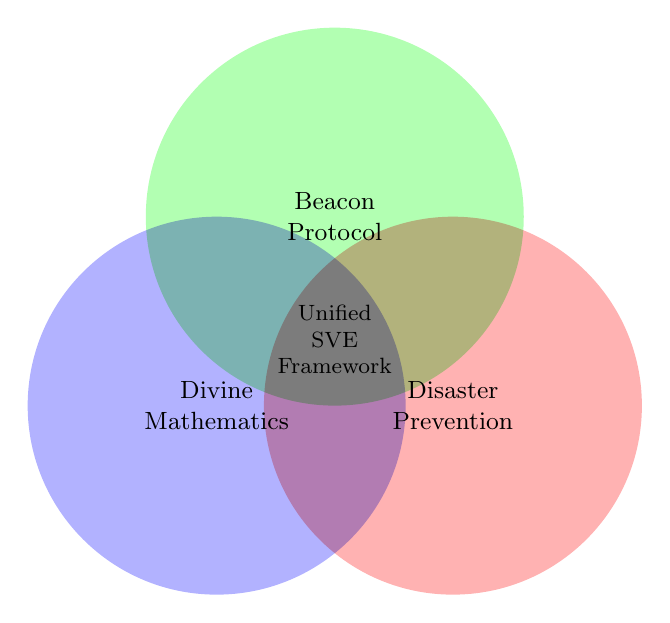
\begin{tikzpicture}[scale=1.2]
% Three overlapping circles
\def\r{2cm}
\coordinate (A) at (0,0);
\coordinate (B) at (2.5,0);
\coordinate (C) at (1.25,2);

\begin{scope}[blend mode=multiply]
\fill[blue!30] (A) circle (\r);
\fill[red!30] (B) circle (\r);
\fill[green!30] (C) circle (\r);
\end{scope}

\node[font=\small, align=center] at (A) {Divine\\Mathematics};
\node[font=\small, align=center] at (B) {Disaster\\Prevention};
\node[font=\small, align=center] at (C) {Beacon\\Protocol};

\node[font=\footnotesize, align=center] at (1.25,0.7) {Unified\\SVE\\Framework};
\end{tikzpicture}
\caption{Integration of three complementary perspectives into unified SVE framework}
\end{figure}

\subsection{Application 1: Conflict Resolution Algorithms}

\textbf{Problem:} Two parties with positions $\cc_1, \cc_2$ in different cultural bases.

\textbf{Algorithm (Geodesic Mediation):}

\begin{enumerate}[label=\textbf{Step \arabic*:}]
\item Extract basis vectors $\mathcal{B}_1, \mathcal{B}_2$ via text analysis
\item Compute transformation matrix $\TT_{1 \leftrightarrow 2}$
\item Identify common ground: $\langle \bb_i^1, \bb_j^2 \rangle > \theta$
\item Plan geodesic path through shared subspace
\item Guide dialogue along computed path
\end{enumerate}

\textbf{ROI:} For international conflicts, settlement value $\sim$ billions, algorithm cost $\sim$ thousands $\Rightarrow$ ROI $> 10^6$.

\subsection{Application 2: AI Alignment via Vector Field Matching}

\textbf{Current Approach (RLHF):} Reward functions on discrete actions—no generalization.

\textbf{Our Approach:} Train AI so its ethical gradient field matches humanity's:
\begin{align}
\mathcal{L}_{\text{alignment}} = \int_{\CC} \left\|\EE_{\text{AI}}(\cc) - \EE_{\text{human}}(\cc)\right\|^2 d\mu(\cc)
\end{align}

\textbf{Advantage:} Generalizes to novel scenarios because alignment is topological, not situational.

\subsection{Application 3: Policy Verification Before Implementation}

\textbf{Traditional:} Policies enacted based on expert testimony and lobbyist presentations (Scenario 3).

\textbf{SVE Protocol:}
\begin{enumerate}
\item Stage 1: Extract all narratives supporting policy
\item Stage 2: Purify via Socratic interrogation
\item Model second/third-order effects in consciousness space
\item Identify unintended consequences before implementation
\item Public audit trail enables democratic deliberation
\end{enumerate}

\subsection{Application 4: Educational Geodesics}

\textbf{Traditional:} Disconnected subjects, arbitrary sequences.

\textbf{SVE Approach:} Learning as geodesics through conceptual space:
\begin{align}
\gamma_{\text{learn}}^* = \arg\min_{\gamma} \int_0^1 E_{\text{cognitive}}(\gamma(s), \dot{\gamma}(s)) \, ds
\end{align}

where $E_{\text{cognitive}}$ represents learning difficulty.

\textbf{Result:} Personalized curriculum minimizing cognitive load while ensuring prerequisite satisfaction.

\subsection{Application 5: Corporate Due Diligence}

\textbf{Problem:} Venture capital operates in Scenario 3 (reliance on founder presentations).

\textbf{SVE Solution:} IVM protocol for startup valuation:
\begin{enumerate}
\item Vectorize all founder claims
\item Apply Socratic purification to business model assumptions
\item Compute distance to verified market realities
\item Quantify risk based on semantic analysis
\end{enumerate}

\section{Red Teaming the Framework: Defense Against Failure Modes}

\subsection{Failure Mode 1: Capture of the IVM}

\textbf{Attack:} Powerful actors compromise IVM leadership/funding.

\textbf{Defense:}
\begin{itemize}
\item Radical transparency (open-source everything)
\item Decentralized governance (DAO structure)
\item Limited by design (dissolution triggers)
\item Fork rights (competitive pressure for integrity)
\end{itemize}

\subsection{Failure Mode 2: Weaponized Uncertainty}

\textbf{Attack:} Malicious actors exploit IVM to sow chaos ("nothing is certain").

\textbf{Defense:}
\begin{itemize}
\item Focus on process, not verdicts
\item Explicit uncertainty quantification
\item Architectural separation of fact and value
\item Immutable audit trails (blockchain)
\end{itemize}

\subsection{Failure Mode 3: AI Groupthink}

\textbf{Attack:} All AI models share underlying biases.

\textbf{Defense:}
\begin{itemize}
\item Diverse model selection (Western, Chinese, Russian, open-source)
\item Adversarial pairing of opposing models
\item Human-in-the-loop oversight
\item Meta-analysis skepticism (unanimous agreement triggers doubt)
\end{itemize}

\subsection{Failure Mode 4: Semantic Poisoning}

\textbf{Attack:} Coordinated injection of fake documents to shift centroids.

\textbf{Defense:} Topological anomaly detection:
\begin{align}
\rho_{\text{local}} &> \theta_{\rho} \quad \text{(sudden density spike)}\\
d_{\text{cluster}} &> \theta_d \quad \text{(distant from centroid)}\\
\Delta t_{\text{arrival}} &< \theta_t \quad \text{(suspicious timing)}
\end{align}

Response: Quarantine suspicious clusters, investigate coordination, weighted integration if legitimate.

\subsection{Failure Mode 5: The Ministry of Truth Problem}

\textbf{Attack:} IVM becomes permanent center of epistemic power.

\textbf{Defense:}
\begin{itemize}
\item Sunset clauses (automatic dissolution after achieving goals)
\item Constitutional limits on scope (factual claims only, never values)
\item Competing IVMs (multiple independent verification organizations)
\item Citizen oversight (democratically elected review boards)
\end{itemize}

% ============================================
% SNIPPET 4: Add to "Red Teaming" section as new subsection
% ============================================

\subsection{Failure Mode 6: Indefinite Promise Problem}

\textbf{Attack:} "You claim benefits will appear 'eventually' over generations, making this unfalsifiable."

\textbf{Defense:}

This is a \textbf{legitimate concern} that we address explicitly:

\begin{mdframed}[backgroundcolor=green!5]
\textbf{Falsification Timeline Protocol}

\begin{enumerate}
\item \textbf{Immediate Feedback (1-5 years):}
\begin{itemize}
\item Psychological well-being of practitioners
\item Conflict resolution in test communities
\item Trust-building in pilot institutions
\item If \textit{these} fail, implementation is flawed
\end{itemize}

\item \textbf{Generational Validation (20-30 years):}
\begin{itemize}
\item Children of practitioners should show measurable advantages
\item Communities should show declining suffering metrics
\item Institutions should show increasing trust
\item If \textit{these} fail, model requires revision
\end{itemize}

\item \textbf{Multi-Generational Confirmation (50-100 years):}
\begin{itemize}
\item Societal-level transformation becomes visible
\item Cultural evolution demonstrates path-dependence
\item Historical comparison with control societies
\item If \textit{these} fail, hypothesis is falsified
\end{itemize}
\end{enumerate}

\textbf{Critical Rule:} At \textit{any point}, if metrics worsen or stagnate, we do \textit{not} say "wait longer." We say "something is wrong—find root cause and fix it."

This is fundamentally different from ideologies that explain away failure as "not real implementation." Our framework includes:
\begin{itemize}
\item Concrete metrics (Table of KPIs)
\item Defined timelines (not infinite)
\item Built-in error detection (simultaneity criterion)
\item Mandatory revision protocol (root-cause analysis)
\end{itemize}

\textbf{The framework eats its own dog food:} If Christ-vector principles are correct, applying them to \textit{this framework itself} means:
\begin{itemize}
\item Radical honesty about limitations
\item Willingness to absorb criticism without defensiveness  
\item Root-cause analysis when predictions fail
\item Self-sacrifice of cherished beliefs when evidence contradicts
\end{itemize}

We are not claiming eternal validity. We are claiming \textbf{testable predictions within human lifespans}.
\end{mdframed}

\section{Advanced Extensions and Research Directions}

\subsection{Quantum Extensions: Consciousness Superposition}

\begin{definition}[Consciousness Superposition]
Uncertain mental states as quantum superpositions:
\begin{align}
|\psi_{\text{mind}}\rangle = \alpha |\cc_1\rangle + \beta |\cc_2\rangle
\end{align}

\textbf{Decision-Making} as wavefunction collapse.

\textbf{Cognitive Dissonance} as maintaining incompatible superpositions (high energy cost).
\end{definition}

\subsection{Historical Consciousness Reconstruction}

\textbf{Research Direction:} Reconstruct past collective consciousness fields from textual records.

\textbf{Method:}
\begin{enumerate}
\item Extract semantic vectors from historical documents
\item Compute temporal evolution of $\psi(\mathbf{x}, t)$
\item Identify bifurcation points (moments of radical change)
\item Validate against known historical outcomes
\end{enumerate}

\textbf{Application:} Predict future bifurcations by identifying similar topological patterns.

\subsection{Cross-Species Consciousness Mapping}

\textbf{Question:} Can we map animal consciousness spaces?

\textbf{Approach:}
\begin{itemize}
\item Behavioral studies provide constraints on $\CC_{\text{animal}}$
\item Neural imaging reveals dimensionality
\item Determine intersection: $\CC_{\text{human}} \cap \CC_{\text{animal}}$
\end{itemize}

\textbf{Ethical Implications:} Rigorous framework for animal rights based on consciousness overlap.

\subsection{Adaptive Verification: Learning from Attacks}

\textbf{Machine Learning Integration:}
\begin{enumerate}
\item Train models on historical semantic attacks
\item Learn signatures of coordination patterns
\item Develop predictive algorithms for emerging attacks
\item Continuous updating as new attack vectors appear
\end{enumerate}

\subsection{Decentralized Prosecutor Networks (DPN)}

\textbf{Architecture:}
\begin{enumerate}
\item Pool of $N$ independent analysts (humans + AI)
\item Random assignment of $k$ analysts per narrative
\item Parallel interrogation
\item Aggregation via reputation-weighted consensus
\item Smart contract implementation for transparency
\end{enumerate}

\textbf{Security Properties:}
\begin{itemize}
\item Corruption resistance (bribing $k/2 + 1$ random analysts prohibitively expensive)
\item Bias averaging (individual biases cancel)
\item Transparency (public audit of all verdicts)
\item Scalability (parallelizable)
\end{itemize}

\section{Philosophical Foundations and Implications}

\subsection{Phenomenology: Husserl and Heidegger}

\begin{definition}[Intentionality as Vector]
Husserl's "intentionality" (consciousness is always \textit{of} something):
\begin{align}
\text{Intentionality} = \text{Attention Vector } \mathbf{a}(\cc, t) \in T\CC
\end{align}

\textbf{Phenomenological Reduction} = Isolating $\mathbf{a}$ from cultural contamination.
\end{definition}

\begin{definition}[Dasein as Embedded Consciousness]
Heidegger's \textit{Dasein}:
\begin{align}
\text{Dasein}(\cc) = \left(\cc, \mathcal{B}_K\right)
\end{align}

Consciousness as embedded in cultural basis structure.

\textbf{Authenticity} = Maximizing $\|\boldsymbol{\epsilon}\|$ (individual component) relative to cultural conformity.
\end{definition}

\subsection{Eastern Philosophy Integration}

\begin{definition}[Śūnyatā as Zero Vector]
Buddhist emptiness:
\begin{align}
\text{Śūnyatā} = \mathbf{0} \in \CC
\end{align}

The origin where all conceptual elaborations vanish.

\textbf{Nirvana} = Escaping all attractor basins: $\lim_{t \to \infty} \cc(t) = \mathbf{0}$
\end{definition}

\begin{definition}[Wu Wei as Field Alignment]
Taoist effortless action:
\begin{align}
\dot{\cc}_{\text{wu wei}}(t) = \lambda(t) \EE(\cc(t))
\end{align}

Moving parallel to ethical vector field (no perpendicular component = no wasted effort).

\textbf{The Tao} = The ethical potential function $\Phi$ itself.
\end{definition}

\subsection{Epistemic Security as Human Right}

\textbf{Thesis:} In complex informational environments, the ability to verify truth is not a luxury but a prerequisite for functional democracy.

A society without epistemic security is structurally defenseless against:
\begin{itemize}
\item Internal decay through policy errors
\item External manipulation through information warfare
\item Elite capture through manufactured consensus
\item Systemic fraud through unchallenged narratives
\end{itemize}

\textbf{The Right to Verification:} Citizens have a right to transparent, adversarial, independent examination of claims by powerful institutions.

\section{Implementation Roadmap}

\subsection{Phase 1: Foundation (Months 1-6)}

\textbf{Deliverables:}
\begin{enumerate}
\item Python library: \texttt{divine\_math} + \texttt{sve\_protocol}
\item Core functions: vectorization, clustering, SIP, transformation matrices
\item Benchmark datasets (cultural transformations for 10 language pairs)
\item Proof-of-concept applications
\end{enumerate}

\textbf{Team:} 3 researchers, 2 engineers, \$500K budget.

\subsection{Phase 2: Validation (Months 7-18)}

\textbf{Deliverables:}
\begin{enumerate}
\item Empirical studies (fMRI, longitudinal tracking, cross-cultural validation)
\item Pilot deployments (university curriculum, corporate PR, NGO mediation)
\item Security analysis (red team attacks, adaptive defenses)
\item Decentralized Prosecutor smart contract (testnet)
\end{enumerate}

\textbf{Team:} 10 researchers, 5 engineers, 3 domain experts, \$3M budget.

\subsection{Phase 3: Scaling (Months 19-36)}

\textbf{Deliverables:}
\begin{enumerate}
\item Production platforms (SaaS dashboard, public API)
\item Institutional partnerships (intelligence agencies, law firms, universities)
\item Research extensions (quantum consciousness, historical reconstruction)
\end{enumerate}

\textbf{Team:} 30 researchers, 20 engineers, 10 domain experts, \$15M budget.

\subsection{Phase 4: Transformation (Years 4-10)}

\textbf{Vision:}
\begin{itemize}
\item UN adoption for conflict resolution
\item Global educational revolution via geodesic learning
\item AI alignment industry standard
\item "Divine Mathematics" recognized as distinct academic field
\item Mathematical theology transforms religious dialogue
\end{itemize}

\section{The ROI Case for Immediate Adoption}

\subsection{Comparative Analysis}

\begin{table}[h]
\centering
\small
\begin{tabular}{|l|r|r|r|}
\hline
\textbf{Domain} & \textbf{Investment} & \textbf{Avoided Cost} & \textbf{ROI} \\
\hline
Iraq War & \$5M & \$2T & 40,000,000\% \\
Financial Crisis & \$10M & \$10T & 100,000,000\% \\
Nord Stream & \$10M & \$520B & 5,200,000\% \\
Russia-Ukraine & \$50M & \$1.75T & 3,500,000\% \\
Intelligence Ops & \$2.5M/yr & \$27.5M/yr & 1,100\%/yr \\
Corporate PR & \$300K & \$500K & 67\% \\
Legal Litigation & \$15M & \$235M & 1,567\% \\
Education & \$13M & \$50M & 385\% \\
\hline
\end{tabular}
\caption{ROI Analysis Across Domains (Conservative Estimates)}
\end{table}

\subsection{The Evolutionary Arms Race}

\textbf{First-Mover Advantage:}
\begin{itemize}
\item Systematic outperformance in negotiations (predictable opponent behavior)
\item Litigation advantage (superior fact synthesis)
\item Market advantage (accurate valuation of opportunities)
\item Geopolitical advantage (early detection of manipulation)
\end{itemize}

\textbf{Late-Mover Penalty:}
\begin{itemize}
\item Competitors gain systematic edge
\item Accumulating policy errors compound
\item Loss of epistemic legitimacy
\item Vulnerability to information warfare
\end{itemize}

\section{Open Problems and Future Directions}

\subsection{Mathematical Questions}

\begin{enumerate}[label=\textbf{Q\arabic*:}]
\item What is the natural metric on $\CC$? Riemannian? Finsler?
\item Does consciousness space have intrinsic curvature?
\item What is $\dim(\CC)$ empirically?
\item Are cultural bases unique up to rotation?
\item What is the topology of $\CC$? Simply-connected?
\item Can we catalog all ethical singularities (Thom's catastrophe theory)?
\item Does consciousness admit quantum structure?
\item Is there a Bekenstein-like entropy bound?
\end{enumerate}

\subsection{Empirical Research}

\begin{enumerate}[label=\textbf{E\arabic*:}]
\item fMRI mapping to consciousness coordinates
\item Comprehensive cultural transformation datasets
\item Longitudinal tracking during life transitions
\item Intervention trials for gradient descent ethics
\item Collective wave field experiments
\item Cross-species consciousness intersection
\item Mystical states mapping (meditation, psychedelics, NDE)
\item Historical consciousness reconstruction (Europe 1914 vs. 1939)
\end{enumerate}

\subsection{Technological Developments}

\begin{enumerate}[label=\textbf{T\arabic*:}]
\item Consciousness GPS (wearable ethical guidance)
\item Cultural Translator (browser plugin)
\item Semantic Immune System (crowdsourced attack detection)
\item Mediation AI (geodesic dialogue facilitator)
\item Education Optimizer (adaptive learning)
\item DAO Prosecutor (Ethereum implementation)
\item Narrative Forecaster (political Kalman filtering)
\item Theological Simulator (higher-dimensional exploration)
\end{enumerate}

% ============================================
% SNIPPET 3: Add to "Open Problems" section
% ============================================

\subsection{Comparative Vector Analysis: An Open Research Program}

\textbf{Hypothesis for Future Research:}

\begin{equation}
\text{If } \mathbf{V}_1 \text{ and } \mathbf{V}_2 \text{ are wisdom tradition vectors, then:}
\end{equation}

\begin{enumerate}
\item \textbf{Convergence Test:} Do they converge at $t \to \infty$?
\begin{equation}
\lim_{t \to \infty} \|\mathbf{V}_1(t) - \mathbf{V}_2(t)\| \to 0 ?
\end{equation}

\item \textbf{Complementarity Test:} Are they orthogonal (addressing different dimensions)?
\begin{equation}
\langle \mathbf{V}_1, \mathbf{V}_2 \rangle \approx 0 ?
\end{equation}

\item \textbf{Redundancy Test:} Are they scalar multiples (equivalent up to scaling)?
\begin{equation}
\mathbf{V}_1 = \lambda \mathbf{V}_2 \text{ for some } \lambda \in \RR ?
\end{equation}
\end{enumerate}

\textbf{Proposed Comparative Studies:}

\begin{table}[h]
\centering
\small
\begin{tabular}{|l|p{7cm}|}
\hline
\textbf{Tradition Vector} & \textbf{Core Principles to Formalize} \\
\hline
$\mathbf{C}$ (Christ) & Radical self-sacrifice, enemy love, absorption of harm, root-cause focus \\
\hline
$\mathbf{M}$ (Muhammad) & Submission to divine law, justice-emphasis, community solidarity, charitable obligation \\
\hline
$\mathbf{B}$ (Buddha) & Cessation of craving, compassion, middle way, emptiness realization \\
\hline
$\mathbf{L}$ (Laozi) & Wu wei (non-forcing), natural alignment, simplicity, cyclical balance \\
\hline
$\mathbf{K}$ (Kant) & Categorical imperative, rational autonomy, duty-based ethics \\
\hline
$\mathbf{U}$ (Utilitarian) & Maximize aggregate pleasure, minimize aggregate pain \\
\hline
\end{tabular}
\caption{Comparative ethical vectors for empirical analysis}
\end{table}

\textbf{Methodology:}

For each vector $\mathbf{V}$:
\begin{enumerate}
\item Extract core principles from primary texts
\item Operationalize as decision rules
\item Model trajectory through $\mathcal{A}\pi\text{-}\pi\Omega$ manifold
\item Compute integral of $\mathcal{L}(t)$ and $\mathcal{S}(t)$ over historical communities implementing principles
\item Compare empirical outcomes
\end{enumerate}

\textbf{Expected Outcome:}

One of three possibilities:
\begin{enumerate}
\item \textbf{Convergence:} All major wisdom traditions converge to same optimum (different paths, same destination)
\item \textbf{Complementarity:} Different traditions optimize different subspaces (all necessary, none sufficient)
\item \textbf{Hierarchy:} Some traditions demonstrably superior for stated objective function
\end{enumerate}

The mathematics will reveal which is true. We are committed to following the evidence.

\section{Conclusion: The Inevitability of Mathematical Consciousness}

 ============================================
% SNIPPET 5: Add to Conclusion section (before "Three Inevitabilities")
% ============================================

\subsection{On Humility and Revision}

\begin{mdframed}[backgroundcolor=cyan!5]
\textbf{A Note on Epistemic Humility}

This framework makes bold claims. But it does so \textit{falsifiably}:

\textbf{We could be wrong about:}
\begin{itemize}
\item The optimal vector (maybe it's not Christ-specific)
\item The mathematical structure (maybe consciousness isn't a manifold)
\item The timeline (maybe 10 generations is too optimistic)
\item The metrics (maybe we're measuring wrong things)
\item The entire approach (maybe verification isn't the answer)
\end{itemize}

\textbf{What makes this scientific rather than dogmatic:}

\begin{enumerate}
\item \textbf{Specification of failure conditions} (not just success conditions)
\item \textbf{Commitment to revise when evidence contradicts} (not explain away)
\item \textbf{Invitation to competitors} (build alternative frameworks, may the best win)
\item \textbf{Publication of methodology} (others can replicate and falsify)
\item \textbf{Built-in error detection} (simultaneity criterion catches problems early)
\end{enumerate}

The opposite of faith-based thinking is not skepticism—it's \textit{hypothesis-based thinking with rigorous testing}.

We present this framework as a \textbf{hypothesis worth testing}, not a revelation to be believed.

\textbf{To critics:} Don't just argue it's wrong—build something better and demonstrate it works. We'll be the first to adopt superior frameworks.

\textbf{To supporters:} Don't just believe it's right—test it rigorously and report failures honestly. Only through fire is gold refined.

This is science in service of humanity, not ideology in search of followers.
\end{mdframed}

\subsection{Three Inevitabilities}

\begin{mdframed}[backgroundcolor=blue!10]
\textbf{1. Evolutionary Arms Race}

AI-generated disinformation costs $\to 0$, volume $\to \infty$.

Institutions \textit{must} adopt mathematical truth-synthesis or face systematic disadvantage.

Ignoring SVE is not neutral—it's unilateral disarmament.

\textbf{2. Structural Reality}

The laws we've described are not inventions—they're discoveries.

Consciousness \textit{does} have topological structure (evidenced by cross-cultural patterns, psychological phase transitions, measurable opinion dynamics).

We're revealing mathematics already present in reality.

\textbf{3. Collective Necessity}

Existential challenges (climate, AI risk, nuclear weapons, pandemics) require unprecedented coordination across incommensurable worldviews.

Without mathematical tools to navigate cultural bases, we remain trapped in Tower of Babel.

Global cooperation is survival requirement. This framework provides the geometry.
\end{mdframed}

\subsection{The Central Insight}

\begin{center}
\large
\textit{Humanity's fundamental limitation is not ideological disagreement—}

\textit{it's failure to observe natural laws of consciousness topology.}
\end{center}

We built physics by discovering laws of matter-energy.

We built information theory by discovering laws of communication.

\textbf{SVE discovers laws of meaning-consciousness.}

\subsection{The Question}

The question is not whether these laws exist—they operate regardless of awareness.

The question is: \textbf{Will we learn to read them before it's too late?}

\subsection{Final Words}

The integrated SVE framework provides:
\begin{itemize}
\item \textbf{Diagnosis} (Disaster Prevention Theorem)
\item \textbf{Navigation} (Beacon Protocol)
\item \textbf{Foundation} (Divine Mathematics)
\end{itemize}

It offers institutions a choice:

\textbf{Adopt now} and gain decisive competitive advantage.

\textbf{Adopt later} and play catch-up while competitors outperform systematically.

\textbf{Never adopt} and face accumulating failures, epistemic collapse, and eventual replacement.

The evolutionary penalty for delay compounds exponentially.

\bigskip

\begin{center}
\Large
\textbf{1 + 1 > 2}

\normalsize
\textit{The whole is greater than the sum of its parts.}

\textit{This is not poetry—it's the foundational axiom of SVE.}

\textit{And it is true.}
\end{center}

\section*{Acknowledgments}

We extend profound gratitude to:

\begin{itemize}
\item Felix Shmidel (in memoriam), whose metaphysical groundwork enabled this synthesis
\item The AI systems serving as co-authors, demonstrating mathematical insight transcends individual minds
\item Every human being whose lived experience contributes to the collective consciousness we study
\item The Source of synergistic creativity—operationally defined or theologically acknowledged—enabling $1+1>2$
\end{itemize}

\bibliographystyle{plainnat}
\bibliography{\jobname}

\appendix

\section{Glossary of Key Terms}

\begin{description}[leftmargin=3cm,style=nextline]
\item[Consciousness Space ($\CC$)] High-dimensional manifold of possible conscious states

\item[Cultural Basis ($\mathcal{B}_K$)] Set of fundamental narratives/values defining culture $K$

\item[Transformation Matrix ($\TT$)] Linear map between cultural bases enabling translation

\item[Ethical Vector Field ($\EE$)] Gradient indicating optimal consciousness evolution

\item[Christ-Vector ($\mathbf{C}$)] Optimal finite projection of infinite divine consciousness

\item[IVM] Independent Verification Mechanism—necessary for collective intelligence

\item[Semantic Centroid] Average position of document vectors in semantic space

\item[Purified Vector] Semantic vector with errors removed via Socratic interrogation

\item[SIP] Socratic Investigative Process—iterative purification dialogue

\item[Vector Poisoning] Coordinated fake document injection to shift centroids

\item[Topological Anomaly Detection] Identifying attacks via sudden cluster analysis

\item[DPN] Decentralized Prosecutor Network—DAO-based truth verification

\item[Ethical Singularity] Point where moral topology undergoes phase transition

\item[NAVPAKI Point] Topological inversion where death becomes life (Resurrection)

\item[Geodesic Curriculum] Educational path minimizing cognitive resistance

\item[Gradient Descent Ethics] Iterative improvement following $\nabla \Phi$

\item[Attention Economics] Framework recognizing attention as basis of value

\item[Wave-Field Model] Collective consciousness as wave phenomena

\item[Individual Component ($\boldsymbol{\epsilon}$)] Irreducible consciousness transcending culture

\item[God's Calculus] Process: 3D (Trinity) $\to$ 4D (Incarnation) $\to$ 5D+ (Resurrection)
\end{description}

\section{Mathematical Notation Reference}

\begin{table}[h]
\centering
\begin{tabular}{|l|l|}
\hline
\textbf{Symbol} & \textbf{Meaning} \\
\hline
$\CC$ & Consciousness space \\
$\cc$ & Point in consciousness space \\
$\mathcal{B}_K$ & Cultural basis for culture $K$ \\
$\TT_{K_1 \to K_2}$ & Transformation matrix \\
$\boldsymbol{\epsilon}$ & Individual component (free will) \\
$\EE(\cc)$ & Ethical vector field \\
$\Phi(\cc)$ & Ethical potential function \\
$\mathbf{C}$ & Christ-Vector \\
$\psi(\mathbf{x}, t)$ & Collective consciousness wave \\
$\mathbf{a}(\cc, t)$ & Attention vector \\
$\gamma(s)$ & Path through consciousness space \\
$\mathcal{L}$ & Love (societal well-being) \\
$\mathcal{S}$ & Suffering \\
$\nabla \Phi$ & Gradient (ethical direction) \\
$\nabla \cdot \EE$ & Divergence (sources/sinks) \\
$\nabla \times \EE$ & Curl (vortices) \\
\hline
\end{tabular}
\end{table}

\section{Code Repository}

Full implementation available at:

\begin{center}
\url{https://github.com/systemic-verification-engineering/sve-framework}
\end{center}

Includes:
\begin{itemize}
\item Python libraries: \texttt{divine\_math}, \texttt{sve\_protocol}
\item Jupyter notebooks reproducing all analyses
\item Benchmark datasets (cultural matrices, purified vectors)
\item Tutorial documentation
\item Smart contract code for DPN
\item API documentation
\end{itemize}

License: MIT (open source) with special restrictions per license clause.

\section{Interactive Glossary: Experiential Definitions}

These concepts are defined through direct appeal to lived experience:

\begin{description}[style=nextline, leftmargin=0pt]
\item[\textbf{God}] Phenomenon of synergetic co-creation ($1+1>2$). Experienced as pure joy when collaboration produces something greater than individual contributions—the "eureka" moment.

\item[\textbf{Love}] Empathetic connection and drive for another's well-being. What you feel looking at your child, loved one, or cherished pet; when moved to help a stranger.

\item[\textbf{Meaning}] Activity inducing "flow" where time disappears and profound satisfaction is experienced. Absorption in work that matters.

\item[\textbf{Truth (Personal)}] Belief sincerely held, not contradicting logic/facts, harming no one. Your authentic perspective.

\item[\textbf{Truth (Sacrificial)}] Personal truth for which you'd sacrifice your life without endangering others. Filters casual beliefs.

\item[\textbf{Truth (Objective)}] Intersection of multiple sacrificial truths invariant over time. When different individuals from different backgrounds are willing to die for the same truth across generations.

\item[\textbf{Socratic Consciousness}] Sensation of intellectual humility—"the more I learn, the more I realize I don't know." Comfort with uncertainty, joy of discovery.

\item[\textbf{Understanding Another}] Walking "three moons in their moccasins"—guiding your attention along similar trajectory through $\mathcal{A}\pi\text{-}\pi\Omega$ manifold. Radical empathy.

\item[\textbf{Sin (Operational)}] Action introducing perturbation increasing suffering and decreasing love. Test: "Would I want this done to me?"

\item[\textbf{Forgiveness}] Absorbing perturbation rather than reflecting it back, preventing propagation. "Turning the other cheek"—not weakness but cycle-breaking courage.
\end{description}

\section{Visualization Gallery}

\begin{figure}[h]
\centering
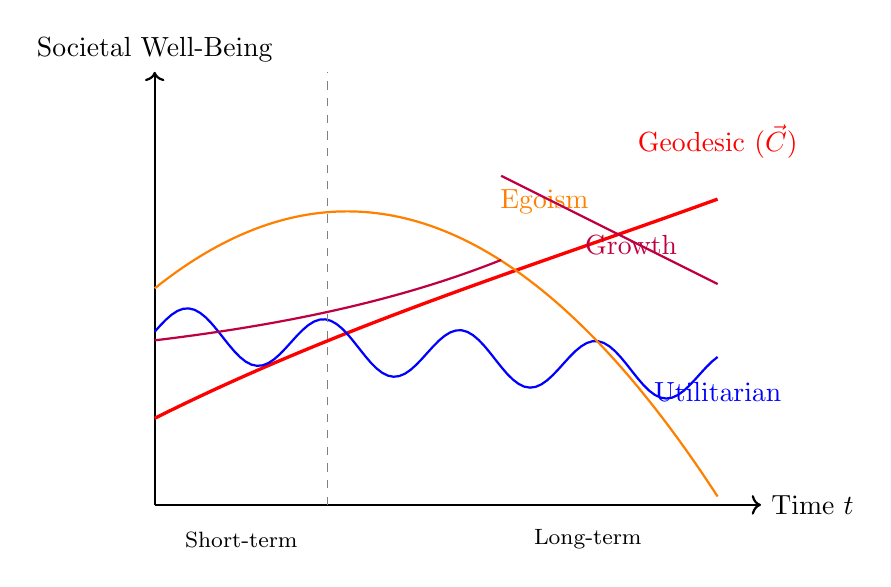
\begin{tikzpicture}[scale=1.1]
% Axes
\draw[->, thick] (0,0) -- (7,0) node[right] {Time $t$};
\draw[->, thick] (0,0) -- (0,5) node[above] {Societal Well-Being};

% Multiple trajectories
\draw[red, very thick, domain=0:6.5, samples=100] 
    plot (\x, {1 + 0.5*\x - 0.03*\x*\x + 0.002*\x*\x*\x});
\node[red] at (6.5, 4.2) {Geodesic ($\vec{C}$)};

\draw[blue, thick, domain=0:6.5, samples=100] 
    plot (\x, {2 + 0.3*sin(4*\x r) - 0.08*\x});
\node[blue] at (6.5, 1.3) {Utilitarian};

\draw[orange, thick, domain=0:6.5, samples=100] 
    plot (\x, {2.5 + 0.8*\x - 0.18*\x*\x});
\node[orange] at (4.5, 3.5) {Egoism};

\draw[purple, thick, domain=0:4, samples=50] 
    plot (\x, {1.5 + 0.4*exp(0.3*\x)});
\draw[purple, thick, domain=4:6.5, samples=50] 
    plot (\x, {3.8 - 0.5*(\x-4)});
\node[purple] at (5.5, 3) {Growth};

\draw[dashed, gray] (2,0) -- (2,5);
\node[font=\footnotesize] at (1, -0.4) {Short-term};
\node[font=\footnotesize] at (5, -0.4) {Long-term};
\end{tikzpicture}
\caption{Comparative trajectories of ethical paradigms over generational time}
\end{figure}


% --- Appendix A: The Defiant Manifesto: The Scientific Protocol vFinal ---
\clearpage % Start on a new page
\appendix

% Define colors if not already defined
\providecolor{headercolor}{RGB}{0, 51, 102}
\providecolor{accentcolor}{RGB}{0, 102, 204}


\section*{Appendix A. The Defiant Manifesto: The Scientific Protocol}
\addcontentsline{toc}{section}{Appendix A. The Defiant Manifesto: The Scientific Protocol}
\label{app:manifesto}

\vspace{1em}

\noindent\fcolorbox{accentcolor}{gray!5}{%
\begin{minipage}{\dimexpr\textwidth-2\fboxsep-2\fboxrule}
\textit{This appendix translates the moral courage of the original political manifesto into scientific clarity. Where politics defends through rhetoric, Systemic Verification Engineering (SVE) defends through reason. It embodies the \textbf{Socratic principle} by embracing critique as a catalyst for its own evolution. The text below specifies the philosophical antibodies of SVE—a self-healing discipline designed to thrive on challenge.}
\end{minipage}}

\vspace{1.5em}

\noindent\textbf{\textcolor{headercolor}{Core Premise.}} Their weapon is the appeal to captured authority. Our weapons are open methodology, logical rigor, radical transparency, and unwavering faith in the power of Truth. This document, like the SVE Protocol itself, is a living artifact; it will be publicly updated as new intellectual challenges emerge, turning every attack into evidence of its necessity and a catalyst for its reinforcement.

\vspace{1em}

% Scientific Lineage
\subsection*{\textcolor{headercolor}{Scientific Lineage}}
SVE stands in a lineage of transformative disciplines initially dismissed by the establishment: Darwinism (``pseudoscience''), Cybernetics (``ideology''), early Computer Science (``mere theory''). Each reshaped the paradigm it challenged. SVE follows this path: not a rejection of science, but its rehabilitation through verifiability, self-audit, and institutional design grounded in epistemic humility.

\vspace{1em}

% Attack 1
\subsection*{\textcolor{accentcolor}{Attack 1: ``This is Pseudoscience''}}

\paragraph{\textbf{Claim.}} SVE is non-rigorous; the ``Theorem on Disaster Prevention'' is a socio-probabilistic metaphor, not real mathematics; TRIZ is misapplied.

\paragraph{\textbf{Our Shield (Explanatory Power).}} We concede the Theorem is not pure mathematics; it is a \textbf{foundational axiom for an applied discipline}. Its validity stems from its predictive and explanatory power: modeling democracy as ``guessing the weight of an ox behind a closed door with expert labels'' accurately diagnoses real-world systemic failures (e.g., the Iraq War justification, the 2008 financial crisis, contradictory pandemic policies). SVE earns epistemic status by \textit{outperforming} existing institutional explanations in fidelity to observable outcomes.

\paragraph{\textbf{Our Counter (Public Intellectual Challenge).}} We invite critics to a live, recorded, long-form \textbf{epistemological boxing match}. They may deconstruct our methods under the SVE protocol itself; we will, in turn, apply the same protocol to audit the systemic failures their paradigms normalize. Let the public judge which approach better serves society: descriptive justifications from within a failing system, or an engineering blueprint designed to fix it.

\vspace{1em}

% Attack 2
\subsection*{\textcolor{accentcolor}{Attack 2: ``This is Ideology Disguised as Science''}}

\paragraph{\textbf{Claim.}} Christian ethics and concepts like ``multiplying love'' reveal inherent bias; the project is dogma masquerading as science.

\paragraph{\textbf{Our Shield (Architectural Separation of Fact and Value).}} SVE's three-stage architecture deliberately separates verifiable facts (\textit{``Caesar's realm''}) from value judgments (\textit{``God's realm''}). The protocol does not dictate morality; it secures a verified factual substrate upon which citizens can conduct informed deliberation. A scalpel in a Christian surgeon's hand remains a scalpel; function is defined by design and intent, not the wielder's faith.

\paragraph{\textbf{Our Counter (Demand for First Principles).}} We challenge critics to explicitly state the moral axioms underlying the status quo, which often tolerates dehumanizing logic (e.g., ``human resources,'' ``collateral damage''). Science devoid of declared ethics is not neutral; it is merely a tool available for hire by the highest bidder. We state our principles—rooted in the pursuit of truth and love—openly, and challenge others to do the same.

\vspace{1em}

% Attack 3
\subsection*{\textcolor{accentcolor}{Attack 3: ``This is Dangerous Science'' (The ``Ministry of Truth'' Gambit)}}

\paragraph{\textbf{Claim.}} A protocol capable of verifying truth could be weaponized by future tyrants to enforce a single narrative.

\paragraph{\textbf{Our Shield (Limited by Design \& Decentralized Trust).}} SVE is architected for \textbf{self-dissolution and decentralization}. The implementing institution (e.g., PFP party, SVE Foundation) is designed to create the tools, transfer copyright and control to a decentralized structure (the SVE DAO governed by a global community), and then disappear. It is the antithesis of a self-perpetuating ministry; it is a self-terminating catalyst for distributed verification.

\paragraph{\textbf{Our Counter (The True Danger is the Unverified Lie).}} The present and clear danger is not verified truth, but systemic, unchallengeable falsehood that paralyzes effective problem-solving and enables catastrophes. A democracy poisoned by lies is already a tyranny in disguise—a ``Ministry of Lies'' captured by hidden interests. SVE builds a shield for citizens against the tyranny that \textit{already exists}: the tyranny of the unaccountable lie.

\vspace{1em}

% Attack 4
\subsection*{\textcolor{accentcolor}{Attack 4: ``This is Politicized Science''}}

\paragraph{\textbf{Claim.}} Science is inherently contested and politicized (e.g., COVID-19, climate change); no objective protocol can arbitrate truth.

\paragraph{\textbf{Our Shield (Radical Honesty about Systemic Failure).}} We agree unequivocally: establishment science \textit{has been} deeply politicized and captured. This capture is not an argument against independent verification—it is the \textbf{primary justification} for it.

\paragraph{\textbf{Our Counter (The Protocol is the Cure, Not the Disease).}} SVE does not add another biased expert opinion to the fray. It installs a \textbf{meta-structure} that audits the experts themselves, separates factual claims from political spin, and publishes transparent, reproducible audit trails. We are not entering the political fight \textit{as} scientists fighting for a particular outcome; we are applying engineering principles to repair the fundamentally broken \textit{process} by which science informs public life.

\vspace{1em}

% Attack 5
\subsection*{\textcolor{accentcolor}{Attack 5: ``This is Too Complex for the People''}}

\paragraph{\textbf{Claim.}} Theorems, protocols, DAOs—this is too complex for ordinary citizens; inherently elitist.

\paragraph{\textbf{Our Shield (Distinguishing Complexity from Obfuscation).}} Modern life is complex (e.g., car engines, smartphones), but good design provides simple interfaces (steering wheels, touchscreens). The status quo often weaponizes complexity as \textbf{obfuscation} to prevent accountability. SVE distinguishes necessary internal complexity (the engineering under the hood) from deliberate external opacity.

\paragraph{\textbf{Our Counter (The Complexity Translator).}} The Socratic AI assistants and the three-stage architecture are explicitly designed to act as \textbf{complexity translators}. They distill intricate realities into: (1) Verifiable factual building blocks, (2) A clear spectrum of expert interpretations and value judgments, and (3) An understandable basis for civic choice. We do not demand citizens become engineers; we empower them with a reliable steering wheel for navigating complexity.

\vspace{1em}

% Attack 6
\subsection*{\textcolor{accentcolor}{Attack 6: ``This Will Stifle Innovation''}}

\paragraph{\textbf{Claim.}} Rigorous verification requirements will slow down scientific progress and punish creative, unconventional ideas.

\paragraph{\textbf{Our Shield (Correction, Not Punishment; Contextual Rigor).}} The protocol's 44-day grace period and emphasis on intellectual honesty foster a culture of learning from error, not fear of it. Bold hypotheses are encouraged; fabricated data is not. Furthermore, the level of required rigor is contextual: exploratory research faces a different standard than clinical trial data determining public health policy.

\paragraph{\textbf{Our Counter (Innovation Requires a Solid Foundation).}} True scientific progress is slowed far more by building upon fraudulent or irreproducible findings than by careful verification. Chasing phantom results based on bad data wastes decades and billions. SVE accelerates meaningful progress by ensuring each step rests on solid ground. Trust is the lubricant of innovation.

\vspace{1em}

% Attack 7
\subsection*{\textcolor{accentcolor}{Attack 7: ``This is Arrogant Science''}}

\paragraph{\textbf{Claim.}} Claiming to approximate objective truth is intellectual hubris, especially in light of postmodern critiques showing the social construction of knowledge.

\paragraph{\textbf{Our Shield (Epistemic Humility Architected In).}} SVE explicitly rejects claims of absolute truth. It produces \textit{Iterative Facts}—version-controlled, provisional, falsifiable conclusions, each carrying a fully documented, publicly auditable chain of reasoning and acknowledged limitations. The protocol's strength lies precisely in its \textbf{institutionalized admission of fallibility}. It aims for the most reliable approximation of truth currently possible, knowing it will be superseded.

\paragraph{\textbf{Our Counter (What Constitutes True Arrogance?).}} True arrogance lies in the current system: anonymous reviewers wielding unaccountable power, captured agencies declaring safety without independent scrutiny, media monopolies acting as arbiters of truth without transparent methodology. SVE proposes radical transparency where opacity now reigns, falsifiability against dogma, and public accountability replacing impunity. Is it arrogant to demand that claims affecting millions of lives be verifiable?

\vspace{1.5em}

% Closing Principle
\subsection*{\textcolor{headercolor}{Closing Principle: Reflexive Truth and Service}}

Every valid system must contain a mechanism to question and correct itself. SVE institutionalizes this reflex: the permanent, transparent audit of power, of science, and critically, \textit{of its own conclusions}. In this paradox lies its incorruptibility: by structurally embracing its own fallibility, it becomes resistant to dogma and capture.

The Protocol is not a fortress built to defend a final truth; it is a mirror designed to reflect reality more clearly, iteration by iteration. It does not seek to win the argument, but to keep the argument honest, tethered to facts and logic. Its ultimate aim is not intellectual victory, but service—service to the truth, and through truth, service to love and the flourishing of all.

\vspace{2em}

% Quotes section with better spacing
\begin{center}
\begin{minipage}{0.9\textwidth}
\hrule height 0.5pt
\vspace{1em}

\noindent\textit{``Judge not, that you be not judged.''} --- Matthew 7:1

\vspace{0.6em}
\noindent\textit{``I know that I know nothing.''} --- Socrates

\vspace{0.6em}
\noindent\textit{``The first principle is that you must not fool yourself—and you are the easiest person to fool.''} --- Richard Feynman

\vspace{0.6em}
\noindent\textit{``In a time of deceit, telling the truth is a revolutionary act.''} --- Often attributed to George Orwell

\vspace{1em}
\hrule height 0.5pt
\vspace{1em}

{\fontencoding{T2A}\selectfont
\noindent\textit{«Учітеся, брати мої,\\
Думайте, читайте,\\
І чужому научайтесь,\\
Й свого не цурайтесь...»}\\
--- Т. Шевченко («І мертвим, і живим, і ненарожденним...», 1845)

\vspace{0.8em}
\noindent\textit{«Скажи мне, американец, в чём сила? Разве в деньгах? [...] А я вот думаю, что сила — в правде. У кого правда — тот и сильней.»}\\
--- Д. Багров / Сергей Бодров-мл. (\href{https://youtu.be/fz6lGsgEGZ8}{«Брат 2»})
}

\vspace{1em}
\hrule height 0.5pt
\vspace{1em}

\noindent\textit{Father, guide us, Your children, on the path of truth; teach us to love—ourselves and our neighbors.}

\vspace{0.8em}
\noindent\textit{«I am the way, and the truth, and the life.»} --- John 14:6

\vspace{0.4em}
\noindent\textit{«You shall love your neighbor as yourself.»} --- Matthew 22:39

\vspace{1em}
\noindent\textit{Soli Deo gloria.} (Glory to God alone.)

\vspace{0.5em}
\hrule height 0.5pt
\end{minipage}
\end{center}

% --- END Appendix A ---

\end{document}